In this section we first explore how well can we approximate variational
expectations in TT format with small ranks.
Then, we compare the proposed TT-GP\footnote{For TT-GP we use our implementation available at
\url{https://anonymized-link}.} method with SVI-GP (\citet{hensman2013}) on regression tasks and KLSP-GP
(\citet{hensman2015}) on binary classification tasks using standard RBF kernel
functions. Then, we test the ability of our method to learn
expressive deep kernel functions and compare it with SV-DKL
(\citet{wilson2016stochastic}).

\subsection{Expectation approximation}
\label{expect_approx}

In this section we provide a numerical justification of using Tensor Train
format for the mean $\mu$ of the variational distribution. We use the Powerplant
dataset from UCI. This dataset consists of $7654$ objects with $4$ features. We place 
$m_0 = 5$ inducing inputs per dimension and form a grid, which gives us a total of $m = 625$
inducing inputs. We train the standard SVI-GP method from GPflow library
(\citet{GPflow2016}) with free form representations for $\mu$ and $\Sigma$.
Then we try to approximate the learned $\mu$ vector with a TT-vector 
$\mu_{TT}$ with small TT-ranks. 

\begin{figure}[!h]
  \vspace{-.3cm}
  \begin{center}
      \begin{tabular}{cc}
          \hspace{-0.3 cm}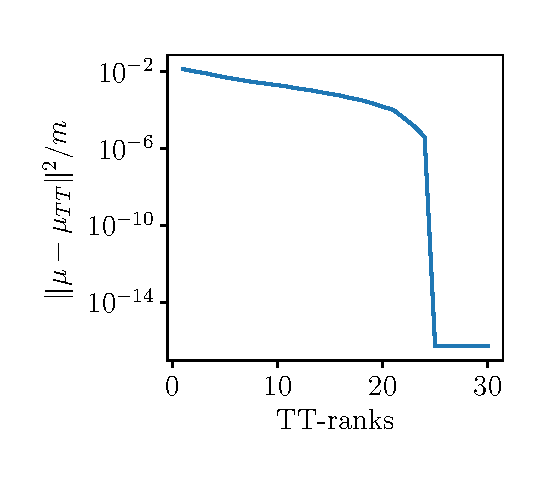
\includegraphics[width=0.5\linewidth]{pics/acc_vs_ranks.eps} &
          \hspace{-0.3 cm}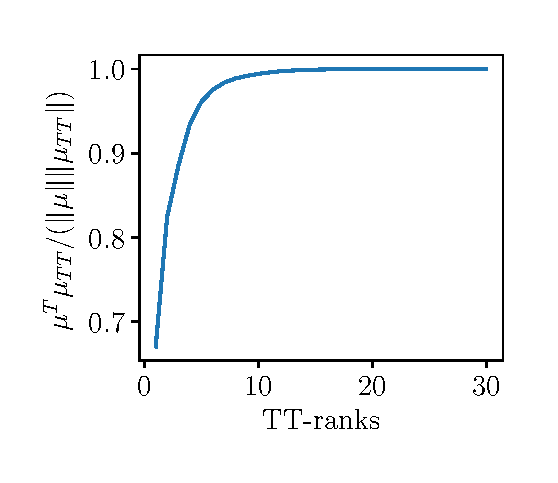
\includegraphics[width=0.5\linewidth]{pics/cos_vs_ranks.eps} \\
          (a) MSE & 
          (b) Cosine similarity
      \end{tabular}
  \end{center}
  \caption{Approximation accuracy as a function of TT-rank.}
  \label{acc_vs_ranks}
\end{figure}

Figure \ref{acc_vs_ranks} shows the dependence between TT-ranks and 
approximation accuracy. For TT-rank greater than $25$ we can approximate the
true values of $\mu$ within machine precision. Note that for TT-rank $25$ the
amount of parameters in the TT representation already exceeds the number of
entries in the tensor $\mu$ that we are approximating. For moderate
TT-ranks an accurate approximation can still be achieved.

\begin{figure}[!h]
  \begin{center}
      \begin{tabular}{cc}
          
\includegraphics[trim = 80 0 80 0, clip, height=0.4\linewidth]{pics/true.eps} &
        \hspace{0.5cm}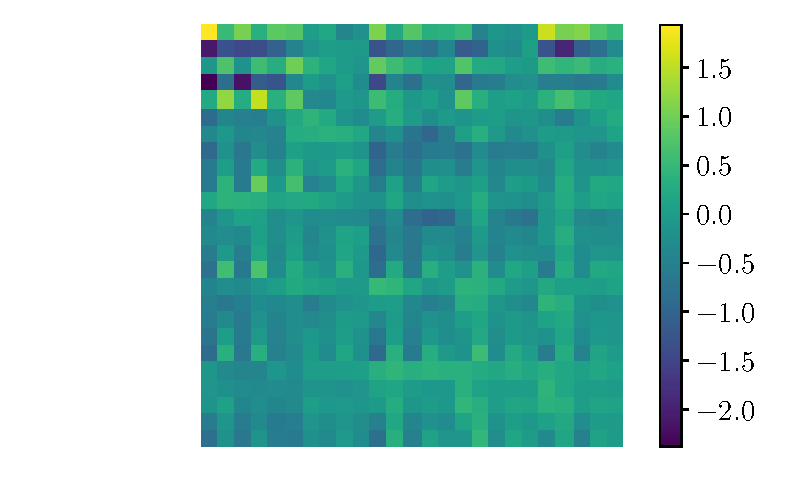
\includegraphics[trim = 80 0 0 0, clip, height=0.4\linewidth]{pics/tt.eps} \\
          (a) $\mu$ &
          (b) $\mu_{TT}$, $r = 10$
      \end{tabular}
  \end{center}
  \vspace{-0.4cm}
  \caption{True variational mean and TT-approximation. Here we reshape the 
    $625$-dimensional $\mu$ and $\mu_{TT}$ vectors
    to $25 \times 25$ matrices for visualization.}
  \label{true_and_tt}
  \vspace{-0.2cm}
\end{figure}

Figure \ref{true_and_tt} shows the true variational mean $\mu$ and it's 
approximation for TT-rank $10$.  We can see that $\mu_{TT}$ captures the 
structure of the true variational mean.

\begin{table*}[!t]
  \caption[]{Experimental results for standard RBF kernels. In the table acc. stands for $r^2$ for regression and accuracy
          for classification tasks. $n$ is the size of the
          training set, $D$ is the dimensionality of the feature space,
          $m$ is the number of inducing inputs, $r$ is TT-ranks of $\mu$ for TT-GP; $t$ is the time per one pass over
          the data (epoch) in seconds; where provided, $d$ is the dimensionality of linear embedding.\\
          $^*$ for KLSP-GP on Airline we provide results from the original
          paper where the accuracy is given as a plot, and detailed
          information about experiment setup and exact results is not available.
          }
  \label{se_results}
  \centering
  \begin{tabular}{lll l cll l cllll}
    \toprule
    \multicolumn{3}{c}{Dataset} && \multicolumn{3}{c}{SVI-GP / KLSP-GP} && \multicolumn{5}{c}{TT-GP} \\
    \cmidrule{1-3}
    \cmidrule{5-7}
    \cmidrule{9-13}

    Name & $n$ & $D$ &&
    acc. & $m$ & $t$ (s) &&
    acc. & $m$ & $r$ & $d$ & $t$ (s)\\
    \midrule

    Powerplant & $7654$ & $4$ &&
    $0.94$ & $200$ & $10$ &&
    $0.95$ & $35^4$ & $30$ & - & $5$ \\

    Protein & $36584$ & $9$ &&
    $0.50$ & $200$ & $45$ &&
    $0.56$ & $30^9$ & $25$ & - & $40$ \\

    YearPred & $463K$ & $90$ &&
    $0.30$ & $1000$ & $597$ &&
    $0.32$ & $10^6$ & $10$ & $6$ & $105$ \\

    \midrule
    Airline & $6M$ & $8$ &&
    $0.665^*$ & - & - &&
    $0.694$ & $20^8$ & $15$ & - & $5200$ \\

    svmguide1 & 3089 & 4 &&
    $0.967$ & $200$ & $4$ &&
    $0.969$ & $20^4$ & $15$ & - & $1$\\

    EEG & 11984 & 14 &&
    $0.915$ & $1000$ & $18$ &&
    $0.908$ & $12^{10}$ & $15$ & $10$ & $10$\\

    covtype bin & 465K & 54 &&
    $0.817$ & $1000$ & $320$ &&
    $0.852$ & $10^6$ & $10$ & $6$ & $172$\\
    \bottomrule
  \end{tabular}
\end{table*}

\subsection{Standard RBF Kernels}

For testing our method with standard RBF covariance functions we used a range of
classification and regression tasks from UCI and LIBSVM archives and the
Airline dataset, that is popular for testing scalable GP models
(\citet{hensman2013}, \citet{hensman2015}, \citet{wilson2016stochastic},
\citet{cutajar2016}).

For SVI-GP and KLSP-GP we used the implementations provided in GPfLow
(\citet{GPflow2016}). For Airline dataset we provide results reported in
the original paper (\citet{hensman2015}). For our experiments, we use a cluster of Intel Xeon E5-2698B v3 CPUs having $16$ cores and $230$ GB
of RAM.

For YearPred, EEG and covtype datasets we used a $d$-dimensional linear embedding inside the RBF kernel for TT-GP, as the number $D$ of features makes it
impractical to set inducing inputs on a grid in a $D$-dimensional space in this case.

  

Table \ref{se_results} shows the results on different regression and
classification tasks. We can see, that TT-GP is able to achieve better
predictive quality on all datasets except EEG. We also note that the
method is able to achieve good predictive performance with linear
embedding, which makes it practical for a wide range of datasets.

\subsection{Deep Kernels}

  \subsubsection{Representation learning}
  We first explore the representation our model learns for data on the small
  Digits\footnote{\url{http://scikit-learn.org/stable/auto_examples/datasets/plot_digits_last_image.html}}
  dataset containing $n = 1797$ $8 \times 8$ images of handwritten digits. We
  used a TT-GP with a kernel based on a small fully-connected neural network
  with two hidden layers with $50$ neurons each and $d = 2$ neurons in the output
  layer to obtain a $2$-dimensional embedding. We trained the model to classify
  the digits to $10$ classes corresponding to different digits.
  Fig. \ref{digits_embedding} (a) shows the learned embedding. We also trained the same
  network standalone, adding another layer with $10$ outputs and softmax
  activations. The embedding for this network is shown in fig. \ref{digits_embedding},b.
\begin{figure}[!t]
  \begin{center}
      \begin{tabular}{c}
          \hspace{-.9cm}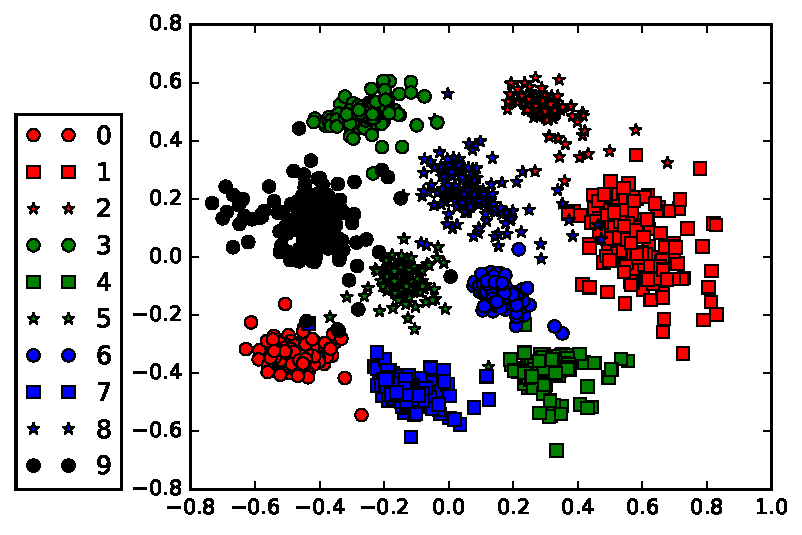
\includegraphics[height=0.45\linewidth]{pics/embedding_ttgp.pdf} \\
          (a) DNN with TT-GP \\
          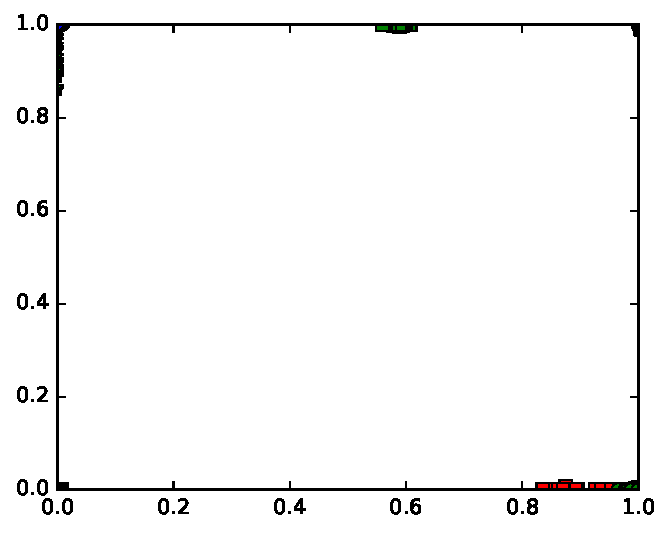
\includegraphics[height=0.45\linewidth]{pics/embedding_dnn.pdf}\\
          (b) Plain DNN\\
      \end{tabular}
  \end{center}
  \vspace{-0.4cm}
  \caption{Learned representation for Digits dataset.}
  \vspace{-0.4cm}
  \label{digits_embedding}
\end{figure}

  \begin{table*}[!t]
    \caption{DNN architecture used in experiments with deep kernels. Here F($h$) means a fully-connected layer with $h$ neurons; C($h{\times}w$, $f$) means a
    convolutional layer with $f$ $h{\times}w$ filters; P($h{\times}w$) means max-pooling with $h{\times}w$ kernel; ReLU stands for rectified linear unit
    and BN means batch normalization (\citet{ioffe2015}).}
    \label{deep_architecture}
    \centering
    \begin{tabular}{ll}
      \toprule
      Dataset & Architecture \\
      \midrule

      Airline & F($1000$)-ReLU-F($1000$)-ReLU-F($500$)-ReLU-F($50$)-ReLU-F($2$)\\

      CIFAR-10 & C($3{\times}3$, 128)-BN-ReLU-C($3{\times}3$, 128)-BN-ReLU-P($3{\times}3$)-C($3{\times}3$, 256)-BN-ReLU-\\
       & C($3{\times}3$, 256)-BN-ReLU-P($3{\times}3$)-C($3{\times}3$, 256)-BN-ReLU-\\
       & C($3{\times}3$, 256)-BN-ReLU-P($3{\times}3$)-F($1536$)-BN-ReLU-F($512$)-BN-ReLU-F($9$)\\

      MNIST & C($5{\times}5$, $32$)-ReLU-P($2{\times}2$)-C($5{\times}5$, $64$)-ReLU-P($2{\times}2$)-F($1024$)-ReLU-F($4$)\\
      \bottomrule
    \end{tabular}
  \end{table*}
  
  \begin{table*}[t]
%    \vspace{-.5cm}
    \caption{Results of experiments with deep kernels. Here acc. is classification
            accuracy; $C$ is the number of classes; $d$ is the dimensionality
            of embedding learned by the model; $t$ is the time per one pass over
            data (epoch) in seconds.}
    \label{deep_results}
    \centering
    \begin{tabular}{llll ll llll lll}
      \toprule
      \multicolumn{4}{c}{Dataset}  && SV-DKL &&
      \multicolumn{2}{c}{DNN} &&
      \multicolumn{3}{c}{TT-GP}\\

      \cmidrule{1-4}
      \cmidrule{6-6}
      \cmidrule{8-9}
      \cmidrule{11-13}

      Name & $n$ & $D$ & $C$ &&
      acc. && acc. & $t$ (s) &&
      acc. & $d$ & $t$ (s)
      \\
      \midrule


      %\cmidrule{9-10}
      %\cmidrule{12-13}

      Airline & $6M$ & $8$ & $2$ &&
      $0.781$ && $0.780$ & $1055$ &&
      $0.788 \pm 0.002$ & $2$ & $1375$\\

      CIFAR-10 & $50K$ & $32{\times}32{\times}3$ & $10$ &&
      $0.770$ && $0.915$ & $166$ &&
      $0.908 \pm 0.003$ & $9$ & $220$\\

      MNIST & $60K$ & $28{\times}28$ & $10$ &&
      $0.992$ && $0.993$ & $23$ &&
      $0.9936 \pm 0.0004$ & $10$ & $64$\\
      \bottomrule
    \end{tabular}
%    \vspace{-.5cm}
  \end{table*}

  We can see that the stand-alone DNN with linear classifiers is unable
  to learn a good $2$-dimensional embedding.
  On the other hand, using a flexible GP classifier that is capable of learning
  non-linear transormations, our
  model groups objects of the same class into compact regions.

  \subsubsection{Classification tasks}
  To test our model with deep kernels we used Airline,
  CIFAR-10 (\citet{krizhevsky2009}) and
  MNIST (\citet{lecun1998}) datasets. The corresponding DNN architectures are shown
  in Table~\ref{deep_architecture}. For CIFAR-10 dataset we also use standard 
  data augmentation techniques with random cropping of $24 \times 24$
  parts of the image, horizontal flipping, randomly adjusting brightness and contrast. In all experiments we also add a BN without trainable mean and
  variance after the DNN output layer to project the outputs into the region
  where inducing inputs are placed. We use $m_0 = 10$ inducing inputs
  per dimension placed on a regular grid from $-1$ to $1$ and set TT-ranks of 
  $\mu$ to $r = 10$ for all three datasets. For experiments with convolutional neural networks, we
  used Nvidia Tesla K80 GPU to train the model.

  Table~\ref{deep_results} shows the results of the experiments for our TT-GP
  with DNN kernel and SV-DKL. Note, that the comparison
  is not absolutely fair on CIFAR-10 and MNIST datasets, as we didn't use
  the same exact architecture and preprocessing as \citet{wilson2016stochastic}
  because we couldn't find the exact specifications of these models.
  On Airline dataset we used the same exact architecture and preprocessing as
  SV-DKL and TT-GP achieves a higher accuracy on this dataset.

  We also provide results of stand-alone DNNs for comparison. We used the
  same networks that were used in TT-GP kernels with the last linear layers replaced
  by layers with $C$ outputs and softmax activations. Overall, we can see, that
  our model is able to achieve good predictive performance,
  improving the results of standalone DNN on Airline and MNIST.

  We train all the models from random initialization without pretraining. We also
  tried using pretrained DNNs as initialization for the kernel of our TT-GP model,
  which sometimes leads to faster convergence, but does not improve the final
  accuracy.
